\documentclass{beamer}
\usetheme{Boadilla}
\usepackage{graphicx}
\usepackage{bbm}
\newcommand{\one}{\mathbbm{1}}
\title[Environmental Activist Investing]{The Real Effects of Environmental Activist Investing}
\subtitle{S. Lakshmi Naaraayanan (LBS), Kunal Sachdeva (Rice), \\Varun Sharma (LBS) \\ 2021 SFS North American Cavalcade}

\author{Alex von Hafften}
\institute{UW-Madison}

\begin{document}

\begin{frame}
\titlepage
\end{frame}


\begin{frame}
\frametitle{Motivation}

\begin{itemize}[<+->]
\item Firms can create negative externalities through environmental impacts.
\begin{itemize}
\item (e.g., toxic chemical release, production emissions, GHG emissions) 
\end{itemize}
\bigskip
\item \textit{Environmental activism} is shareholders engaging with management about environmental impact of their firm.
\bigskip
\item Environmental activism is growing.
\bigskip
\item What are the real effects of environmental activism on targeted firms and their environmental impacts?
\end{itemize}

\end{frame}


\begin{frame}
\frametitle{Approach}
\begin{itemize}[<+->]
\item Naaraayanan et al (2021) evaluates the effects of the Boardroom Accountability Project (BAP).
\bigskip
\item They use a difference-in-differences specification to estimate the effectiveness of climate-focused engagements.
\end{itemize}
\end{frame}


\begin{frame}
\frametitle{Main Results}
\begin{itemize}[<+->]
\item Targeted firms reduced emissions.
\begin{itemize}
\item Reduce toxic chemical release by average of 13\%.
\end{itemize}
\bigskip
\item Reduced negative externalities on local populations.
\bigskip
\item Due to improved abatement initiatives - not reduced production.
\bigskip
\item Abatement hurts the target firms' financial performance.
\end{itemize}
\end{frame}

\begin{frame}
\frametitle{Related Literature}
\begin{itemize}[<+->]
\item Mature literature on shareholder activism affecting corporate governance, financial performance, and operational performance.
\begin{itemize}
\item Nesbitt (1994), Smith (1996), Wahal (1996), Huson (1997), Carleton, Nelson, and Weisbach (1998), Del Guercio and Hawkins (1999).
\end{itemize}
\bigskip
\item Growing literature on investor preferences for socially responsible investments.
\begin{itemize}
\item Atta-Darkua and Dimson (2019), Becht et al (2019), Broccardo et al (2020), Chowdry et al (2018), Hart and Zingales (2017), Morgan and Tumlinson (2019), Oehmke and Opp (2020).
\end{itemize}
\bigskip
\item This paper fills gap on how shareholders can influence corporate environmental behavior, impacts on local populations, and implications on financial performance.
\end{itemize}
\end{frame}


\begin{frame}
\frametitle{Boardroom Accountability Project (BAP)}
\begin{itemize}[<+->]
\item The New York City Pension System initiated BAP on November 4th, 2014.
\bigskip
\item Goal was to hold corporate boards of portfolio companies more accountable to long-term shareholders about certain issues.
\begin{itemize}
\item Board diversity, climate change risks, employee treatment, and excessive CEO pay.
\end{itemize}
\bigskip
\item Without prior announcement, BAP submitted proposals requesting proxy access bylaws be added to targeted firms' corporate charters.
\bigskip
\item These proposals posed a credible threat that long-term shareholders could nominate directors to the boards.
\bigskip
\item Naaraayanan et al (2021) focus on firms targeted based on environmental reasons.
\end{itemize}
\end{frame}

\begin{frame}
\frametitle{Data}

\begin{center}
\begin{tabular}{ l | l}
\textbf{Description} & \textbf{Source}\\ 
\hline
Targeted firms  & BAP  \\  
\hline
Standard firm-level data & Compustat, CRSP, ISS, ASSET4  \\
\hline
Plant-level emissions data & TRI and GHGRP from EPA \\
\hline
Plant ownership & FOIA request\\
\hline 
Local pollutant intensity & RSEI from EPA \\
\hline
Outdoor air quality  & AQS \\
\hline
Plant-level electric output  & EIA
\end{tabular}
\end{center}
\end{frame}


\begin{frame}
\frametitle{Target Selection}
Estimate probability of selection as target firm using logit regression:
\begin{align*}
P(Environment_i) = \Lambda(& \beta_1 \one(Fossil Free_{i}) + \beta_2 Firm \; Size_{i,t-1} \\&+ \beta_3 Market \; to \; Book_{i,t-1} + \beta_4 Returns_{i,t-1} \\&+ \beta_5 Profitability_{i,t-1} + \beta_6 Institutional \; Ownership_{i,t-1} \\&+ \beta_7 ASSET4 \; Score_{i,t-1})
\end{align*}

\begin{itemize}[<+->]
\item $\one(Environment_i)$ equals one if the BAP targets firm $i$.
\item $\one(Fossil Free_{i})$ equals one if firm $i$ within top 100 coal and top 100 oil and gas publicly traded reserve holders.
\item $Firm \; Size_{i,t}$ is log book asset of firm $i$ in year $t$.
\item $Market \; to \; Book_{i,t}$ is market equity plus book debt over book assets.
\item $Returns_{i,t}$ is stock return in past 12 months.
\item $Profitability_{i,t}$ is EBITDA over sales.
\item $Institutional \; Ownership_{i,t}$ is \% of shares held by institutional investors.
\item $ASSET4 \; Score_{i,t}$ is environmental rating by Thomson Reuters
\end{itemize}

\end{frame}

\begin{frame}
\frametitle{Target Selection Results}
\centering
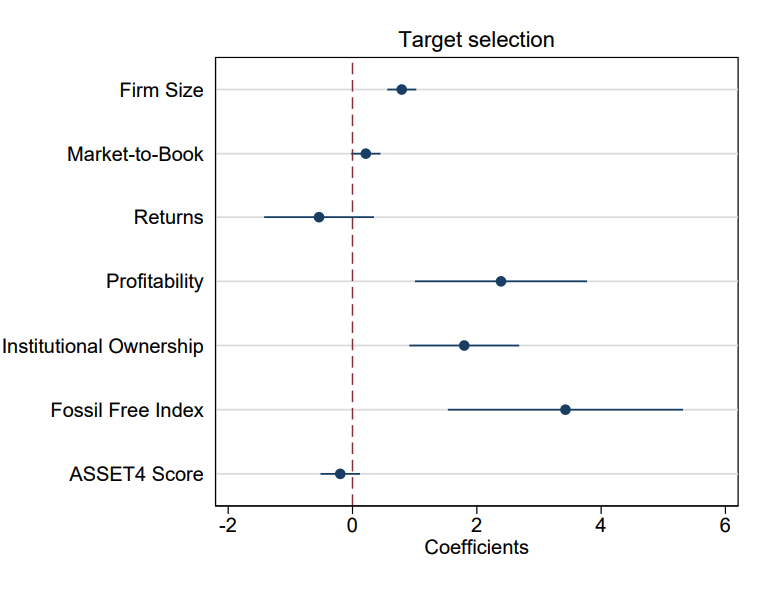
\includegraphics[scale = .25]{target_selection}

\end{frame}


\begin{frame}
\frametitle{Propensity Score Matching}

\begin{itemize}[<+->]
\item Estimate propensity of being targeted by BAP from logit regression.
\bigskip
\item Match each targeted firm in industry $j$ and year $t$ with the untargeted firm in industry $j$ and year $t$ with the closest propensity score.
\bigskip
\item Within industry matching controls for aggregate industry-level trends (e.g., changes in oil prices).
\end{itemize}


\end{frame}

\begin{frame}
\frametitle{Difference-in-Differences Specification}

Use difference-in-differences specification to compare plants of targeted firms to plants of a matched control firm:

\begin{align*}
Y_{i,c,t} &= \beta_1 \one(Post_{i,t}) + \beta_2 \one(Post_{i,t}) \one(Environment_i)+\delta_{i,c} + \delta_{c,t} + \varepsilon_{i,c,t}
\end{align*}

\begin{itemize}[<+->]
\item $Y_{i,c,t}$ is the outcome associated with chemical or gas $c$ emitted by a plant $i$ at time $t$.
\item $\one(Post_{i,t})$ equals one for plant-years following BAP targeting.
\item $\one(Environment_i)$ equals one if the BAP targets the firm.
\item $\delta_{i,c}$ and $\delta_{c,t}$ are plant-chemical and chemical-time FEs, respectively.
\end{itemize}

\bigskip

$\implies \beta_2$ is coefficient of interest.

\end{frame}

\begin{frame}
\frametitle{Reduction in Toxic Chemical Release}

\scriptsize
$$
Y_{i,c,t} \equiv \log\Bigg(1 + \frac{Emission_{i,c,t}}{COGS_{i,t}}\Bigg)
$$

\centering
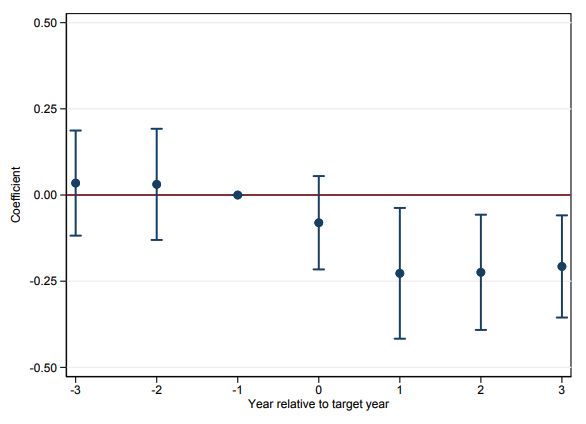
\includegraphics[scale=0.45]{pollution}
\end{frame}


\begin{frame}
\frametitle{Reduction in Toxic Chemical Release}
{
\centering
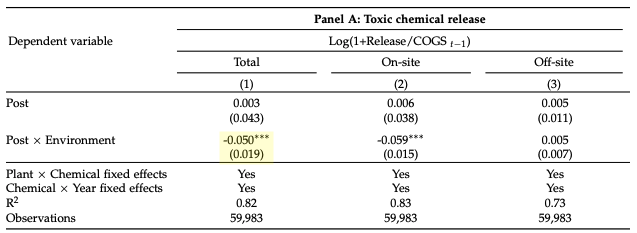
\includegraphics[scale=0.45]{pollution_table}
}
\bigskip

This estimate represents a decrease of 13 \% relative to the sample mean emission.
\end{frame}


\begin{frame}
\frametitle{Reduction in Pollution}

Results generally hold across types of pollutants:

\bigskip

\begin{itemize}[<+->]
\item $\beta_2$ is negative for total and on-site chemical release and insignificant for off-site. No evidence of moving chemicals off-site.
\bigskip
\item $\beta_2$ is negative for stack air (intended release), fugitive emissions (leaks), and surface water discharges.
\bigskip
\item $\beta_2$ is negative for most GHG emissions (methane and nitrous oxide; insignificant for carbon dioxide).
\end{itemize}
\end{frame}


\begin{frame}
\frametitle{Reduction in Negative Environmental Externalities}
\begin{itemize}[<+->]

\item Fewer emissions of chemical associated with respiratory, developmental, nervous system, hematologic (blood-related), and hepatic (liver-related) damage to humans.
\bigskip
\item Improvements in air quality (less ozone, sulfur dioxide and particulate matter) around plants.
\bigskip
\item Evidence that reductions near population centers are significant.
\end{itemize}
\end{frame}

\begin{frame}
\frametitle{How are firms reducing pollution?}
No evidence of firms reducing production.
\bigskip

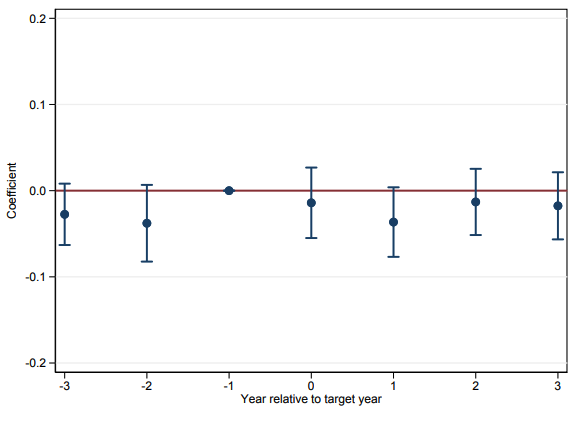
\includegraphics[scale=0.4]{production}

\bigskip

Dependent variable is usage of chemical $c$ in $t$ relative to usage of chemical $c$ in first year of the sample.
\end{frame}


\begin{frame}
\frametitle{How are firms reducing pollution? }
Firms increased abatement efforts.

\bigskip

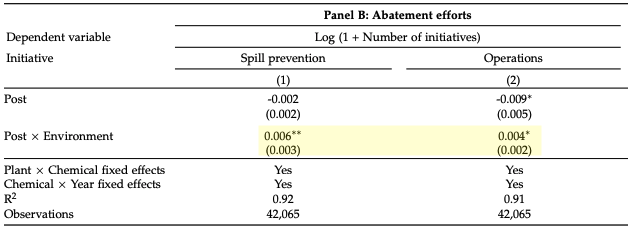
\includegraphics[scale=0.45]{abatement_table}

\bigskip

These estimates represent a 30\% increase in abatement initiatives relative to the sample mean.

\end{frame}

\begin{frame}
\frametitle{Do the increased abatement costs potential financial benefits in the short-run?}

Naaraayanan et al (2021) document two financial outcomes for firms targeted by BAP.

\begin{itemize}[<+->]
\item Neutral equity response.
\item Negative relationship between environmental improvements and financial performance.
\end{itemize}
\end{frame}

\begin{frame}
\frametitle{Neutral Equity Response}

No change in cumulative abnormal returns around announcement date.

\bigskip
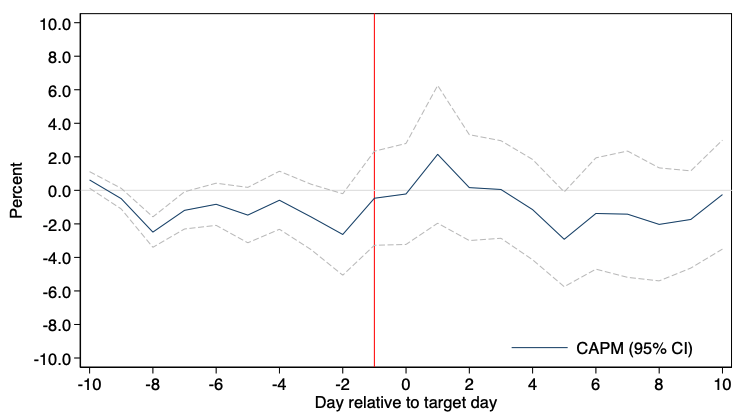
\includegraphics[scale=0.3]{equity_response}
\bigskip

Interpretation: Investor perceive the benefit of increased sustainability balance the higher costs.
\end{frame}



\begin{frame}
\frametitle{Negative Financial Performance}
Targeted firms saw
\begin{itemize}[<+->]
\item Lower return on assets
\item Lower profitability (proxy for financial performance)
\item No change to Z-score (proxy for distress risk)
\end{itemize}
\bigskip
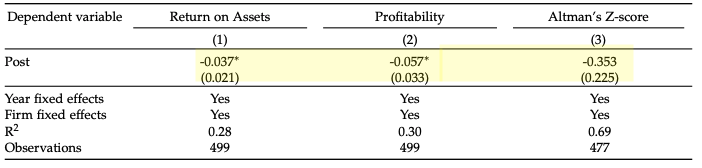
\includegraphics[scale=0.4]{financial_performance}

\end{frame}



\begin{frame}
\frametitle{Weaknesses}

\begin{itemize}[<+->]
\item Their approach estimates the treatment effect on the treated.
\bigskip
\item They discuss effects on ``local economies" a lot, but they're focus is pollution effects on local populations. Not evaulating at local economic outcome...
\bigskip
\item Need model to evaluate the net benefits (how to evaluate non-pecuniary benefits).
\bigskip
\item Robustness: Try synthetic control instead of propensity score matching.
\end{itemize}

\end{frame}


\begin{frame}
\frametitle{Weaknesses (con't)}

\begin{itemize}[<+->]
\item Some skepticism about applicability of propensity score matching.
\bigskip
\item Summary statistics from appendix:
\end{itemize}

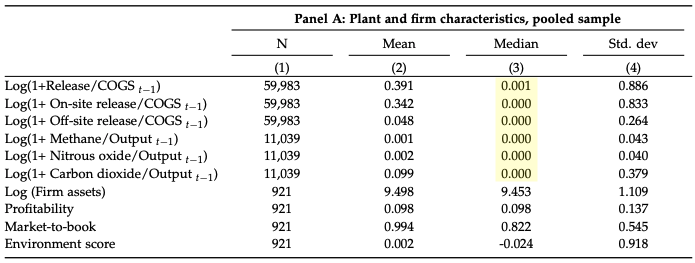
\includegraphics[scale=0.4]{skewness}

\begin{align*}
Median(\log(1+Release/COGS)) &= 0\\
\implies Median(Release) &= 0 \\
\implies \text{Half the sample has no emissions}&
\end{align*}

\end{frame}

\begin{frame}
\frametitle{New Questions}

\begin{itemize}[<+->]
\item All results (pollution, financial performance) are all short-term. What are longer-term effects?
\bigskip
\item How to evaluate net benefits of environmental activism?
\bigskip
\item How to think about agency conflicts regarding environmental impacts between shareholders and management?
\bigskip
\item What are the impacts on firms targeted for non-environment reason by the BAP?
\begin{itemize}
\item E.g. Did board diversity change at firms targeted for a lack of diversity?
\end{itemize}
\end{itemize}

\end{frame}

\end{document}

